\documentclass[12pt, a4paper, oneside]{ctexart}

\usepackage{graphicx}
\usepackage[top=1.5in, bottom=1in, left=1in, right=1in]{geometry}
\CTEXsetup[format={\Large\bfseries}]{section}

\pagestyle{plain}
\linespread{1.5}
\setlength{\parindent}{0pt}
\begin{document}

  \begin{center}
    \textsc{\Large{2023华中师范大学 菜鸟杯 新生程序设计竞赛\\}}
    \fontsize{10mm}{7mm}\selectfont
    \textbf{\Large{参赛手册\\
    }}
  \end{center}

  \section{比赛时间}
  2023 年 12 月 17 日 \ 10: 00 - 15: 00
  \section{比赛地点}
  华中师范大学桂子山校区 \  9号教学楼三楼机房
  
  \begin{center}
    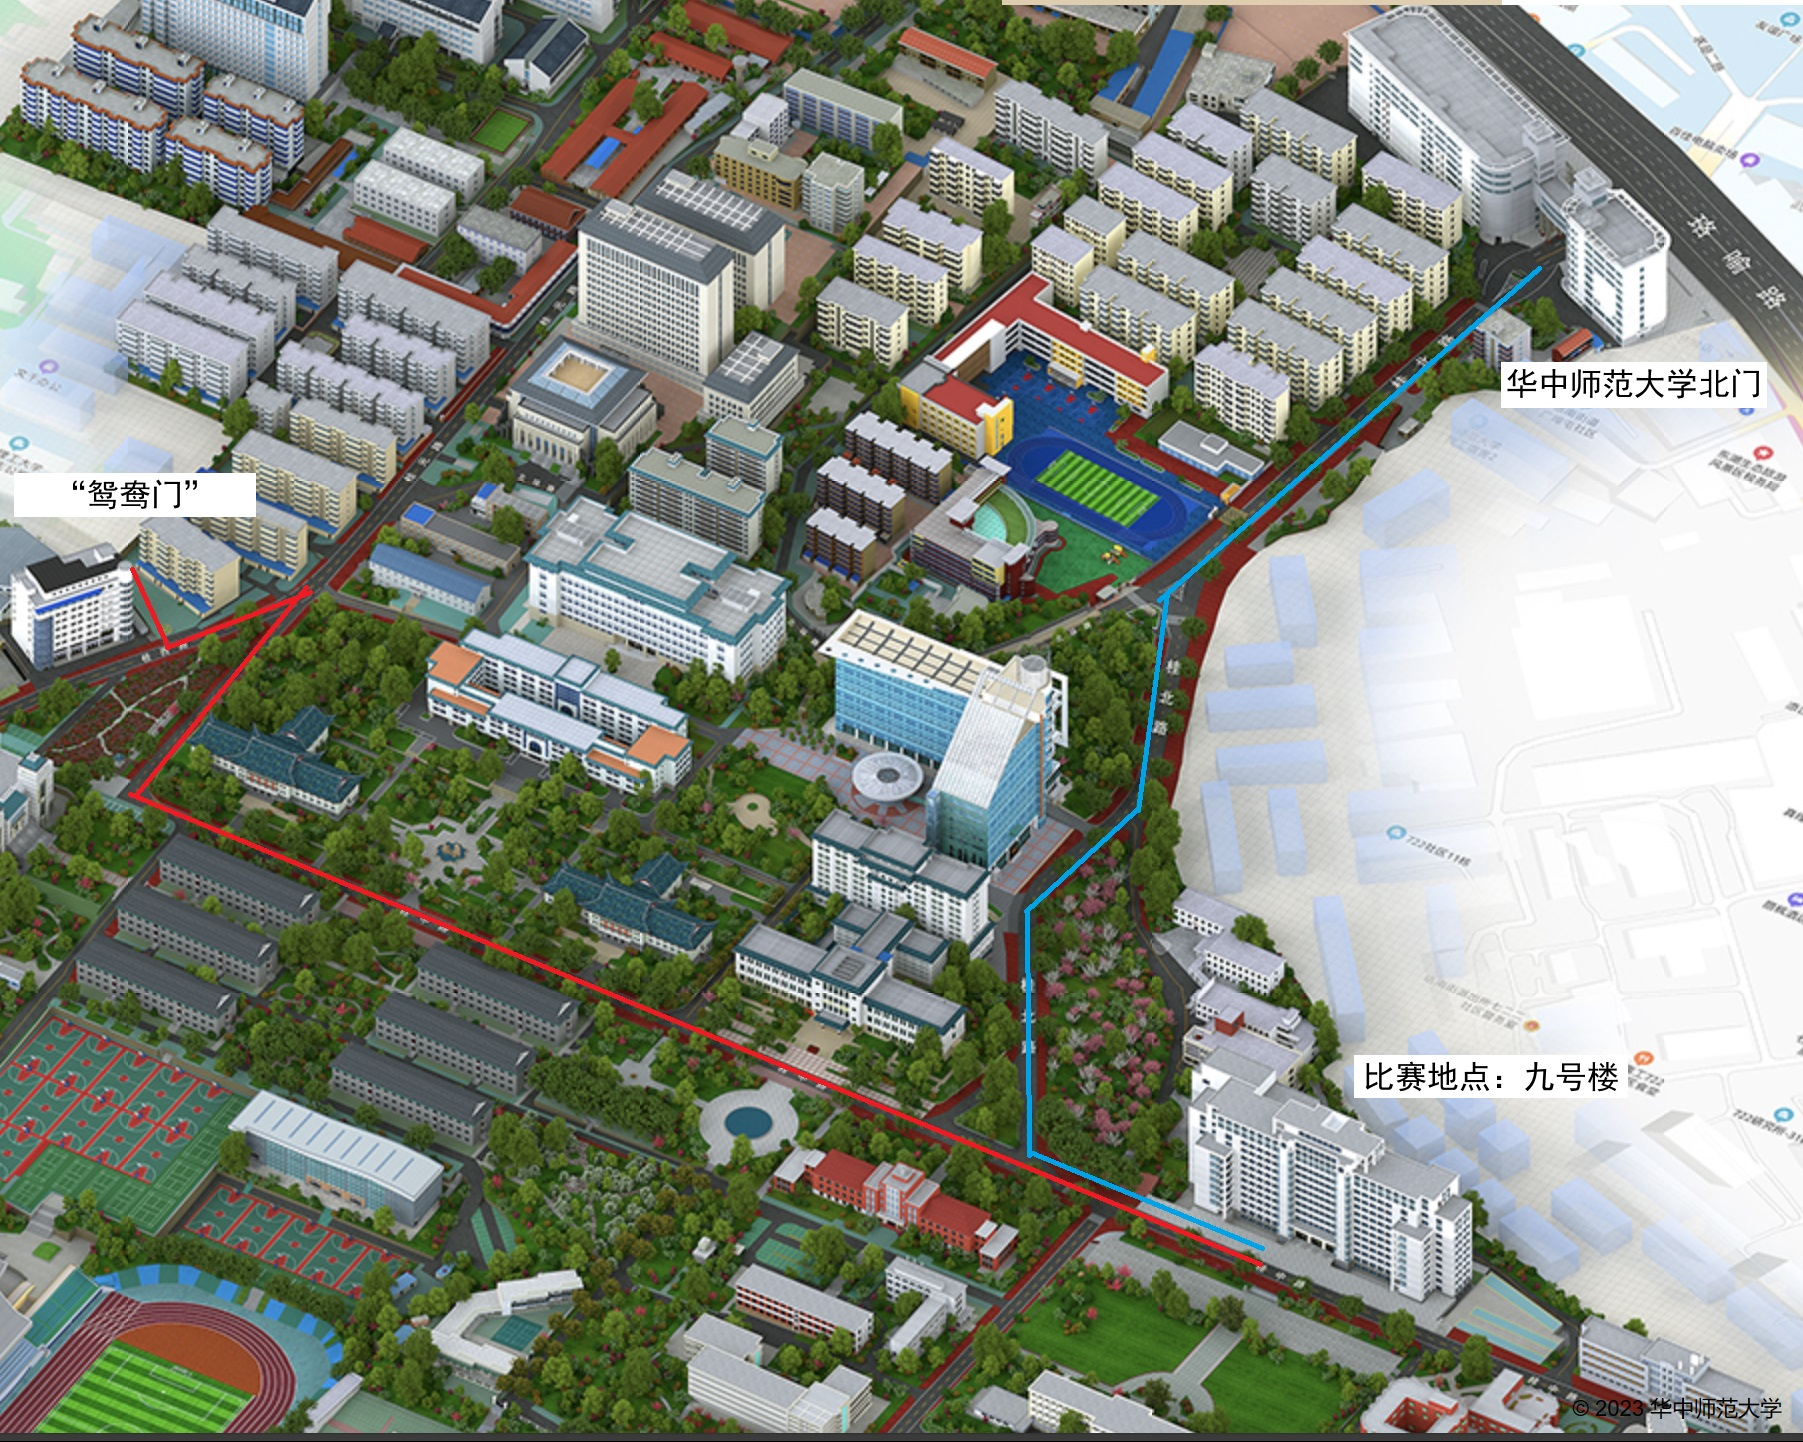
\includegraphics[height=12cm]{route.jpg}
  \end{center}
  
  \section{外校选手注意}
  应校方要求,外校选手请于周日早上 9: 20 前在华中师范大学桂子山
  校区北门外集合,由工作人员带队,核验身份后进入学校。请参赛选
  手务必携带身份证,准时在北门集合。\\
  路线: 行至地铁二号线广埠屯站A出口或公交珞喻路广埠屯站即达北门。

  \section{线上同步赛}
  https://ac.nowcoder.com/acm/contest/72445

  \section{比赛环境}
  评测机环境: \\
  DOMjudge 8.2\\
  GCC (C++20,O2 优化) \ OpenJDK \ Python 3.12\\
  本地环境: 
  Windows 10\\
  编辑器: VSCode (含 C++,Java,Python 插件), 记事本\\
  C++: CLion, DevC++\\
  Java: IntelliJ IDEA\\
  Python: PyCharm\\
  安装的编译器: 与评测机保持一致, 请以实际为准。
  \section{奖项设置}
  一等奖: 校内一名,校外一名。奖品: 蓝牙耳机\\
  二等奖: 校内两名,校外两名。奖品: 机械键盘\\
  三等奖: 校内五名,校外五名。奖品: 鼠标\\
  最佳女生奖: 校内一名。\\
  颁奖仅针对线下参赛选手,牛客同步赛视为打星参赛。
  \section{特别提醒}
  1. 赛中会给参赛选手提供午餐。\\
  2. 选手可以携带翻阅纸质资料,但不能使用自带键盘、蓝牙鼠标等外接设备,手机、耳
  机等电子设备。\\
  3. ACM 赛制个人赛,最后一小时封榜。
  





  \begin{figure*}[b]
    \centering{
      {\large{华中师范大学 ACM 程序设计协会\\  2023/12/17}}\\
    }
  \end{figure*}
\end{document}